%TODO Figure 4: trajectories are not continuous because of snipping them. That's why a red traj is red and outside the collision area.

\section{Recurrent Neural Network: Binary classification} \label{sec:rnn_clf}

\subsection{Introduction}

Recurrent Neural Networks (RNNs) have been shown to extract sequential information and generate highly complex sequences as documents, translations, music and more. In comparison to n-gram models, which have been used in language model for speech recognition, a RNN makes a prediction by a high-dimensional interpolation between training samples. N-gram models predict by creating a distribution, based on the number of exact matches between the recent history and the training set (graves). 


\begin{figure}
	\centering
	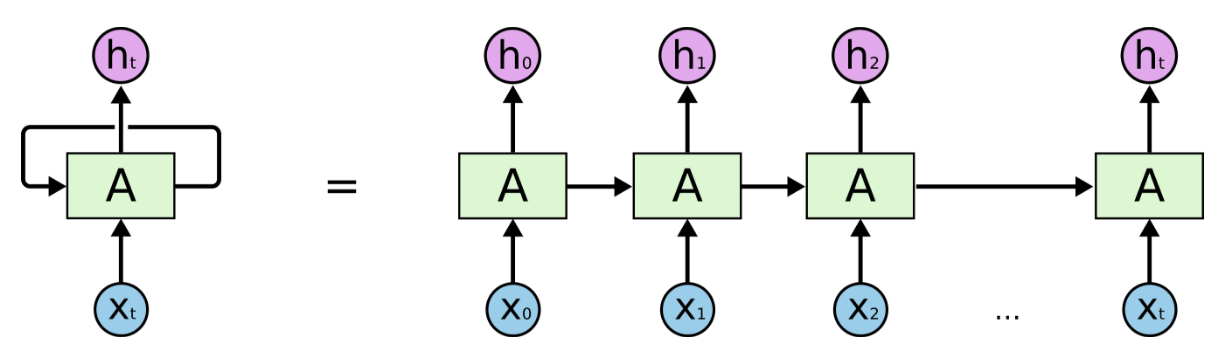
\includegraphics [trim=0 0 0 0, clip, angle=0, width=0.8\columnwidth,
	keepaspectratio]{figures/rnn_unrolled}
	\caption{Illustration of a RNN in it's enrolled (left) and unrolled (right) form. Each sequential input $x_t$ is fed in at timestep $t$, transformed by the activation cell $A$ and output and fed into the next cell as hidden state $h_t$. (colah)} 
	\label{fig:rnn_unrolled} 
\end{figure}

In theory RNNs can be trained by backpropagating the error along the chain of cells. However, every step involves a multiplication with the weight matrix $W$, which, in many cases, results in either an exploding or vanishing gradient (see class exercise). The exploding gradient problem is, in practice, leveraged by gradient clipping (cs232 lecture). The $\textit{vanishing gradient problem}$ is leveraged by a specific architecture of RNNs, called $\textit{Long Short-term Memory}$ (LSTM) networks. They are splitting up the RNNs hidden state into a hidden and a cell state, whereas the cell state, like ResNets, is updated by a sum-operation, rather than a whole transformation (SEE FIGURE ... for the comparison of RNN to LSTM cell). The gradient along a sum-operation splits up equally and thereby allows to propagate until the beginning of the sequence without vanishing.

\begin{figure}
	\centering
	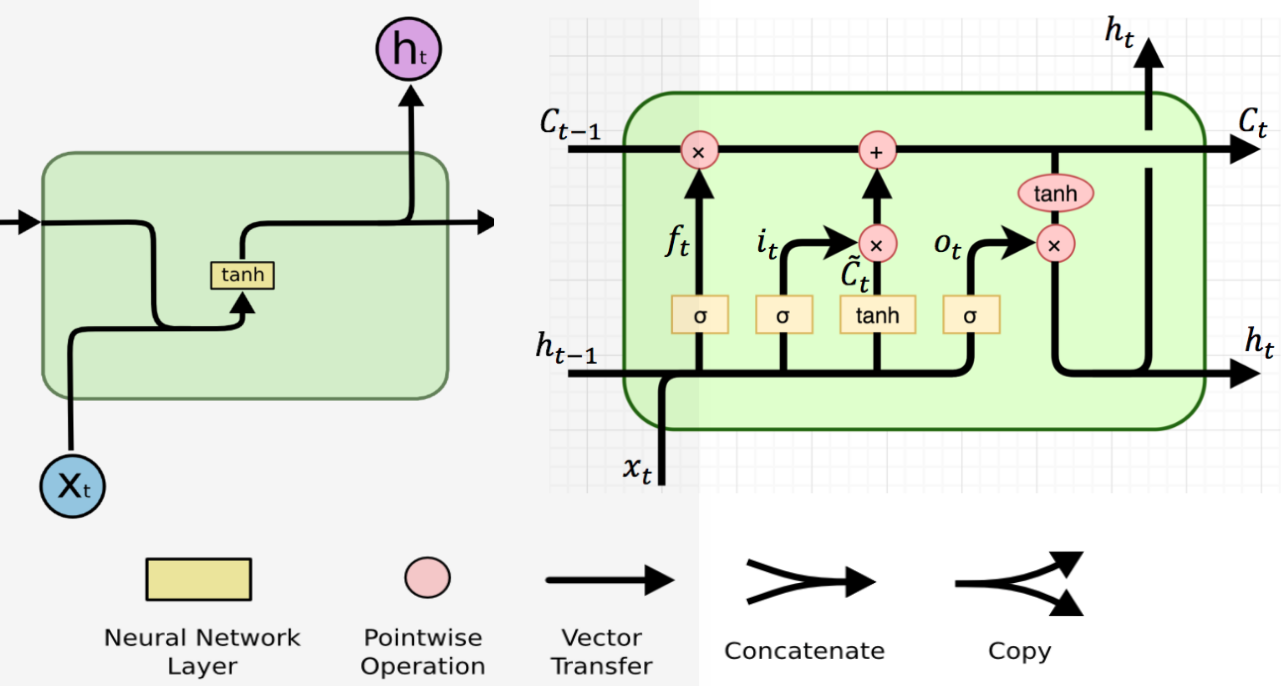
\includegraphics [trim=0 0 0 0, clip, angle=0, width=1.0\columnwidth,
	keepaspectratio]{figures/rnn_lstm}
	\caption{Activation cell of a traditional RNN (top) and a LSTM (bottom). LSTM propagates the cell $c_t$ and hidden $h_t$ state. With ignoring the forget gate $f_t$, $c_t$ is only updated by sum operations. The gradient along a sum-operation splits up equally and thereby allows to propagate until the beginning of the sequence without vanishing. ResNets have introduced a similar change in the CNN architecture (resnet paper). (changhau)} 
	\label{fig:rnn_lstm} 
\end{figure}

%TODO take graph of graves paper.
The LSTM is computed according to the following composite function (graves):
\begin{equation}
\begin{aligned}
& i_t = \sigma(W_{xi}x_t + W_{hi}h_{t-1} + W_{ci}c_{t-1} + b_i)\\
& f_t = \sigma(W_{xf}x_t + W_{hf}h_{t-1} + W_{cf}c_{t-1} + b_f)\\
& c_t = f_tc_{t-1} + i_ttanh(W_{xc}x_t + W_{hc}h_{t-1} + b_c)\\
& o_t = \sigma(W_{xo}x_t + W_{ho}h_{t-1} + W_{co}c_{t-1} + b_o)\\
& h_t = o_ttanh(c_t)
\end{aligned}
\label{eq:lstm_eq} 
\end{equation}
where $\sigma$ is the sigmoid function, $i_t$, $f_t$, $o_t$ and $c_t$ are the input gate, forget gate, output gate and cell activation vectors. All weight matrices have the same meaning, for example $W_{hf}$ is the hidden-forget weight matrix. For clarity, bias terms are omitted. Figuratively speaking, the input gate regulates how much information is taken from the new input $x_t$. The forget gate can erase the cell memory and thereby shorten or lengthen the time dependency of a sequence prediction. The cell state is the propagated memory. The output gate regulates how much information from the hidden cell state is propagated into the output hidden state.

\subsection{LSTMs for binary classification}
We have used LSTM networks for the same binary classification task, as for SVMs. LSTMs are able to extract the sequential information and should thereby provide better classification accuracy in the train and test dataset. All calculations have been done in python and the network has been set up with the $\textit{tensorflow}$ library.

The full trajectories have been precompiled into sniplets of static sequence length $T$. At each time step, the input vector is the relative pedestrian position at time $t$: $x_t \in \Re^{1x2}$. For binary classification, we use a many-to-one architecture. The output is calculated at the output layer by using a logistic sigmoid for binary classification:

\begin{equation}
y_t = \sigma(W_{hout}h_t + b_out)
\label{eq:bin_class_out} 
\end{equation}
where $y_t \in [0,1]$ and $W_{hout} \Re^(n_{hidden} x 1)$, where $n_{hidden}$ is the number of hidden units. The weight matrices and biases are initialized with random noise $N(0,1)$. The loss is computed with least mean squared error (LMSE). The system is optimized by a stochastic gradient descent (SGD) method with the goal to minimize the loss over the weight matrices and their biases.

\subsubsection{Hyperparams in bin class}
- Optimize number of hidden units
- batchsize
- learning rate
- maximum epochs
 


- challenge: predict real-valued sequence
- low dimensionality and ease of visualization
- no sophisticated preprocessing or feature-extraction techniques (graves p.18)
	- reduce variation in data (normalize character size, slant, skew,)
- Compare our dataset to handwritten dataset size (graves p.18)
- handwriting has 25 timesteps per character and 700 timesteps per line
- 5000 training, two val of 1500 lines, test 4000 lines (each line 700 tsteps)
